\documentclass[a4paper,fleqn,12pt]{article}
\usepackage[utf8]{inputenc}
\usepackage[bulgarian]{babel}
\usepackage{amsmath}
\usepackage{amssymb}
\usepackage{booktabs}
\usepackage{fancyhdr}
\usepackage{amsthm}
\usepackage{graphicx}
\usepackage{listings}
\usepackage{xcolor}

\lstset{
    language=Java,         % Choose the language of the code
    basicstyle=\ttfamily\small,  % Code font and size
    keywordstyle=\color{blue},   % Keywords color
    commentstyle=\color{green},  % Comments color
    stringstyle=\color{red},     % Strings color
    numbers=none,                % Line numbers on the left
    breaklines=true,             % Automatic line breaking
    frame=single,                % Add a frame around the code
    showstringspaces=false,  % Prevents spaces in strings from being shown as visible markers
}

\begin{document}
\begin{titlepage}
	\setlength{\parindent}{0pt}
	\large
\centering
Технически университет - София \par
Факултет по Приложна Математика и Информатика \par
\vspace{2cm}

{\huge Задача \par}

\vspace{2cm}

\vspace{1cm}
{\LARGE\scshape  Имплементация на AVL дърво \par}

\vfill
\begin{minipage}[t]{.5\linewidth}
	Студент: Кристиян Кръчмаров \\
	Фак. номер: 791324005
\end{minipage}
%\begin{minipage}[t]{.5\linewidth}
%	\raggedleft
%
%\end{minipage}

\vspace{2cm}
\raggedright

\end{titlepage}
\pagenumbering{gobble}
\tableofcontents
\newpage
\pagenumbering{arabic}
\newpage

\section{Какво е AVL дърво?}
AVL дървото е вид балансирано двоично дърво за търсене, при което за всеки възел разликата във височините на лявото и дясното поддърво е най-много 1. 
Това свойство го прави самобалансиращо се, което гарантира че операциите по добавяне, търсене и изтриване ще се изпълнят с еднаква сложност $O(\log n)$, където n са броят възли на дървото.  \\
За първи път AVL дървото е споменато през 1962 година, когато двама руски учени, Георгий Аделсон-Велски и Евгений Ландис, публикуват статия, в която описват концепцията за самобалансиращо се двоично дърво за търсене.
Името на AVL дървото идва от първите букви на техните фамилии: Adelson-Velsky и Landis. \\
\section{Реализация}
За реализацията е използван програмният език Java. За улеснение е реализирано обикновенно двоично дърво за търсене (Binary search tree) което е надградено, за да се получи AVL дървото.

\subsection{Връх}
Реализиран е клас \texttt{Node} който е POJO (Plain Old Java Object) в който има само информация за един връх, неговата стойност, неговия родител и неговите две деца (ляво и дясно) 
\begin{lstlisting}
public class Node {
    public Integer value;
    public Node parent;
    public Node left;
    public Node right;

    public Node(Integer value, Node parent, Node left, Node right) {
        this.value = value;
        this.parent = parent;
        this.left = left;
        this.right = right;
    }
}
\end{lstlisting}

\subsection{Обикновенно двоично дърво за търсене}
Реализиран е абстрактен клас BinarySearchTree в който са имплементирани основни функционалностти като добавяне, търсене и изтриване от дървото, като и помощни функционалностти като представяне на дървото в конзолата.  \\
\\
В този клас има променливи за коренът на дървото както и за броя елементи. Има абстрактен метод за създаване на връх, който трябва да бъде дефиниран в класа на AVL дървото, защото върхът в AVL дървото има допълнителен параметър за височина, която е разстоянието от възела до най долния лист.  
\begin{lstlisting}
public abstract class BinarySearchTree {
    protected Node root;

    protected int size;

    protected abstract Node createNode(int value, Node parent, Node left, Node right);
\end{lstlisting}
Mетода\texttt{ search} търси възел със стойност element в дървото като започва от корена и в зависимост от стойността се избира левия или десния клон. 
\begin{lstlisting}
protected Node search(int element) {
        Node node = root;
        while (node != null && node.value != null && node.value != element) {
            if (element < node.value) {
                node = node.left;
            } else {
                node = node.right;
            }
        }
        return node;
    }
\end{lstlisting}
\newpage
\noindent 
Метода \texttt{insert} добавя нов елемент в дървото. 
Ако няма корен го добавя като такъв. 
Ако има корен се търси подходяща позиция на която да бъде добавен новия елемент като дете.
\begin{lstlisting}
protected Node insert(int element) {
        if (root == null) {
            root = createNode(element, null, null, null);
            size++;
            return root;
        }

        Node insertParentNode = null;
        Node searchTempNode = root;
        while (searchTempNode != null && searchTempNode.value != null) {
            insertParentNode = searchTempNode;
            if (element < searchTempNode.value) {
                searchTempNode = searchTempNode.left;
            } else {
                searchTempNode = searchTempNode.right;
            }
        }

        if (insertParentNode == null) {
            return null;
        }

        Node newNode = createNode(element, insertParentNode, null, null);
        if (insertParentNode.value > newNode.value) {
            insertParentNode.left = newNode;
        } else {
            insertParentNode.right = newNode;
        }

        size++;
        return newNode;
    }
\end{lstlisting}
\newpage

\noindent 
Метода \texttt{delete} служи за изтриване на връх със стойност element и заменянето му с друг елемент от дървото. 
\begin{lstlisting}
 protected Node delete(int element) {
        Node deleteNode = search(element);
        if (deleteNode != null) {
            return delete(deleteNode);
        } else {
            return null;
        }
    }

protected Node delete(Node deleteNode) {
        if (deleteNode != null) {
            Node nodeToReturn = null;
            if (deleteNode.left == null) {
                nodeToReturn = transplant(deleteNode, deleteNode.right);
            } else if (deleteNode.right == null) {
                nodeToReturn = transplant(deleteNode, deleteNode.left);
            } else {
                Node successorNode = getMinimum(deleteNode.right);
                if (successorNode.parent != deleteNode) {
                    transplant(successorNode, successorNode.right);
                    successorNode.right = deleteNode.right;
                    successorNode.right.parent = successorNode;
                }
                transplant(deleteNode, successorNode);
                successorNode.left = deleteNode.left;
                successorNode.left.parent = successorNode;
                nodeToReturn = successorNode;
            }
            size--;
            return nodeToReturn;
        }
        return null;
    }
\end{lstlisting}
\newpage    

\noindent
Методът \texttt{transplant} служи за заменяне на възел (nodeToReplace) с нов възел (newNode).
\begin{lstlisting}
private Node transplant(Node nodeToReplace, Node newNode) {
        if (nodeToReplace.parent == null) {
            this.root = newNode;
        } else if (nodeToReplace == nodeToReplace.parent.left) {
            nodeToReplace.parent.left = newNode;
        } else {
            nodeToReplace.parent.right = newNode;
        }
        if (newNode != null) {
            newNode.parent = nodeToReplace.parent;
        }
        return newNode;
    }
\end{lstlisting}
Методът \texttt{print} отпечатва дървото в конзолата.
\begin{lstlisting}
public void print() {
        printSubtree(root);
    }
\end{lstlisting}
Методът \texttt{printSubtree} отпечатва първо дясното поддърво за дадения връх, след което принтира стойността на върха, чрез printNodeValue и след това принтира лявото подддърво. \\
Методът \texttt{printNodeValue} отпечатва стойноста на върха в зависимост дали я има. \\
Mетодът \texttt{printTree} е рекурсивен метод който отпечатва дървото с индентация. 
Ако има дясно поддърво се извиква printTree като се увеличават отстъпите. 
Отпечатва се съответната стойност и взависимост и в зависимост дали е дясно или ляво дете се слага съответно "/" или "$\backslash$". 
След това се отпечатва лявото поддърво ако го има. 
\begin{lstlisting}
private void printSubtree(Node node) {
        if (node.right != null) {
            printTree(node.right, true, "");
        }
        printNodeValue(node);
        if (node.left != null) {
            printTree(node.left, false, "");
        }
    }
\end{lstlisting}

\begin{lstlisting}
private void printNodeValue(Node node) {
        if (node.value == null) {
            System.out.print("<null>");
        } else {
            System.out.print(node.value);
        }
        System.out.println();
    }

private void printTree(Node node, boolean isRight, String indent) {
        if (node.right != null) {
            printTree(node.right, true, indent + (isRight ? "        " : " |      "));
        }
        System.out.print(indent);
        if (isRight) {
            System.out.print(" /");
        } else {
            System.out.print(" \\");
        }
        System.out.print("----- ");
        printNodeValue(node);
        if (node.left != null) {
            printTree(node.left, false, indent + (isRight ? " |      " : "        "));
        }
    }
\end{lstlisting}

\newpage

\subsection{Връх в AVL дърво}
Класът \texttt{AVLNode} е разширение на класа \texttt{Node} като добавя полето \texttt{height}.
\begin{lstlisting}
public class AVLNode extends Node {
    public int height;

    public AVLNode(int value, Node parent, Node left, Node right) {
        super(value, parent, left, right);
    }
}
\end{lstlisting}

\subsection{AVL дърво}
В класът \texttt{AVLTree} са доразвити някои от методите в \texttt{BinarySearchTree} и е имплементиран метода \texttt{createNode} 
\begin{lstlisting}
public class AVLTree extends BinarySearchTree {
    @Override
    protected Node createNode(int value, Node parent, Node left, Node right) {
        return new AVLNode(value, parent, left, right);
    }
\end{lstlisting}
Методите за добавяне и изтриване на елемент използват методите реализирани в \texttt{BinarySearchTree} и след извършване на съответното действие, дървото се балансира чрез метода \texttt{balanceTree}. 
\begin{lstlisting}
@Override
public Node insert(int element) {
    Node newNode = super.insert(element);
    balanceTree((AVLNode) newNode);
    return newNode;
}
\end{lstlisting}
\newpage
\begin{lstlisting}
@Override
public Node delete(int element) {
    Node deleteNode = super.search(element);
    if (deleteNode != null) {
        Node successorNode = super.delete(deleteNode);
        if (successorNode != null) {
            AVLNode minimum = successorNode.right != null ? (AVLNode) getMinimum(successorNode.right) : (AVLNode) successorNode;
            recomputeHeight(minimum);
            balanceTree((AVLNode) minimum);
        } else {
            recomputeHeight((AVLNode) deleteNode.parent);
            balanceTree((AVLNode) deleteNode.parent);
        }
        return successorNode;
    }
    return null;
}
\end{lstlisting}
Един от основните методи в AVL дървото е \texttt{balanceTree} който служи за балансиране на дървото при добавяне и изтриване на елементи. 
В този метод се обхожда всеки един връх. За текущ връх се пресмятат височините на поддърветата му,  след това се изчислява фактора на баланс. 
\begin{itemize}
\item Ако факторът е равен на 2, то дясното поддърво е по високo и трябва да се провери
	\begin{itemize}
	\item Ако дясното поддърво е пряко (дясното поддърво на дясното поддърво е ненулево). Тогава се извършва ляво въртене. 
	\item Ако дясното дърво е криво (лявото поддърво на дясното поддърво е ненулево). Тогава се извършва двойно въртене (първо дясно въртене, след това ляво въртене). 
	\end{itemize}
\item Ако факторът е равен на -2, то лявото поддърво е по високо и трябва да се провери.
	\begin{itemize}
	\item Ако лявото поддърво е пряко (лявото поддърво на лявото поддърво е ненулево). Тогава се извършва завъртане на дясно.
	\item Ако лявото поддърво е криво (дясното поддърво на лявото поддърво е ненулево). Тогава се извършва двоен двойно въртене (първо ляво въртене, след това дясно въртене).
	\end{itemize}
\end{itemize}
\begin{lstlisting}
    private void balanceTree(AVLNode node) {
        while (node != null) {
            Node parent = node.parent;

            int leftHeight = (node.left == null) ? -1 : ((AVLNode) node.left).height;
            int rightHeight = (node.right == null) ? -1 : ((AVLNode) node.right).height;
            int nodeBalance = rightHeight - leftHeight;

            if (nodeBalance == 2) { //  2 means right subtree overgrow
                if (node.right.right != null) {
                    node = (AVLNode) avlRotateLeft(node);
                    break;
                } else {
                    node = (AVLNode) doubleRotateRightLeft(node);
                    break;
                }
            } else if (nodeBalance == -2) { // -2 means left subtree overgrow          
                if (node.left.left != null) {
                    node = (AVLNode) avlRotateRight(node);
                    break;
                } else {
                    node = (AVLNode) doubleRotateLeftRight(node);
                    break;
                }
            } else {
                updateHeight(node);
            }

            node = (AVLNode) parent;
        }
    }
\end{lstlisting}
\newpage
\noindent 
Двата метода \texttt{rotateLeft} и \texttt{avlRotateLeft} са двата основни метода за извършване на лява ротация или LL ротация. Метода \texttt{rotateLeft} извършва основната ротация, а \texttt{avlRotateLeft} извиква метода \texttt{rotateLeft} както и метода за промяна на височината на съответните възли. 
\begin{lstlisting}
private Node rotateLeft(Node node) {
        Node temp = node.right;
        temp.parent = node.parent;

        node.right = temp.left;
        if (node.right != null) {
            node.right.parent = node;
        }

        temp.left = node;
        node.parent = temp;
        if (temp.parent != null) {
            if (node == temp.parent.left) {
                temp.parent.left = temp;
            } else {
                temp.parent.right = temp;
            }
        } else {
            root = temp;
        }
        return temp;
    }

private Node avlRotateLeft(Node node) {
        Node temp = this.rotateLeft(node);

        updateHeight((AVLNode) temp.left);
        updateHeight((AVLNode) temp);
        return temp;
    }
\end{lstlisting}
\newpage
\noindent 
Аналогично методите \texttt{rotateRight} и \texttt{avlRotateRight} извършват дясна ротация или RR ротация. 
\begin{lstlisting}
private Node rotateRight(Node node) {
        Node temp = node.left;
        temp.parent = node.parent;

        node.left = temp.right;
        if (node.left != null) {
            node.left.parent = node;
        }

        temp.right = node;
        node.parent = temp;
        if (temp.parent != null) {
            if (node == temp.parent.left) {
                temp.parent.left = temp;
            } else {
                temp.parent.right = temp;
            }
        } else {
            root = temp;
        }
        return temp;
}

private Node avlRotateRight(Node node) {
        Node temp = this.rotateRight(node);

        updateHeight((AVLNode) temp.right);
        updateHeight((AVLNode) temp);
        return temp;
}
\end{lstlisting}
\noindent
Методите \texttt{doubleRotateRightLeft} и \texttt{doubleRotateLeftRight} използват методите \texttt{avlRotateRight} и \texttt{avlRotateLeft}, за да извършат двойните ротации, а именно дясно-лявата RL ротация и ляво-дясната LR ротация.
\newpage 
\begin{lstlisting}
private Node doubleRotateRightLeft(Node node) {
        node.right = avlRotateRight(node.right);
        return avlRotateLeft(node);
    }

private Node doubleRotateLeftRight(Node node) {
        node.left = avlRotateLeft(node.left);
        return avlRotateRight(node);
    }
\end{lstlisting}
Meтодите \texttt{recomputeHeight}, \texttt{maxHeight} и \texttt{updateHeight} се използват за актуализация на височините на възлите в дървото.  \\
\texttt{recomputeHeight} обновявава височините на всички възли, \texttt{maxHeight} пресмята максималната височина между два възела, \texttt{updateHeight} актуализира височината на даден възел спрямо децата му.
\begin{lstlisting}
private void recomputeHeight(AVLNode node) {
        while (node != null) {
            node.height = maxHeight((AVLNode) node.left, (AVLNode) node.right) + 1;
            node = (AVLNode) node.parent;
        }
}
private int maxHeight(AVLNode node1, AVLNode node2) {
        if (node1 != null && node2 != null) {
            return Math.max(node1.height, node2.height);
        }
        if (node1 == null) {
            return node2 != null ? node2.height : -1;
        }
        if (node2 == null) {
            return node1 != null ? node1.height : -1;
        }
        return -1;
}
private void updateHeight(AVLNode node) {
        int leftHeight = (node.left == null) ? -1 : ((AVLNode) node.left).height;
        int rightHeight = (node.right == null) ? -1 : ((AVLNode) node.right).height;
        node.height = 1 + Math.max(leftHeight, rightHeight);
}
\end{lstlisting}
\newpage
\section{Демо}
За демонстрация на имплементацията на AVL дърво ще използваме следния код
\begin{lstlisting}
public static void main(String[] args) {
        AVLTree tree = new AVLTree();
        Random rand = new Random(42);
        for (int i = 0; i < 15; i++) {
            int i1 = rand.nextInt(15);
            if (!tree.contains(i1)) {
                tree.insert(i1);
                System.out.println("Inserted: " + i1);
                tree.print();
                System.out.println();
            }
        }
    }
\end{lstlisting}
Този код инициализира обект tree от клас \texttt{AVLTree}. 
След това се взимат 15 произволни числа от 0 до 15. Проверява дали вече има такъв елемент в дървото, ако няма то този елемент бива добавен. 
Изпечатва се кой е добавения елемент и се изпечатва дървото.  
\begin{figure}[h!]
	\centering
        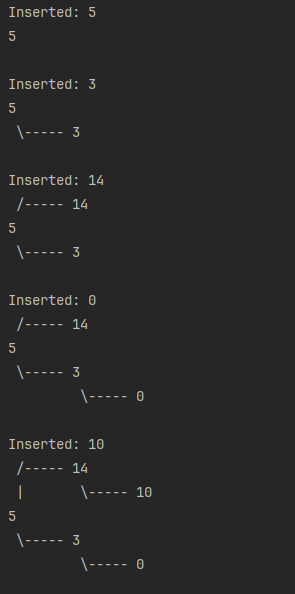
\includegraphics[scale=0.53]{images/result1.png}
        \caption{Първи 5 добавяния в дървото}
\end{figure}
\newpage
\begin{figure}[h!]
	\centering
        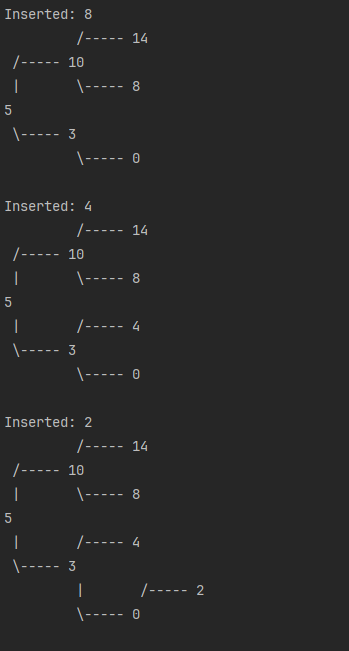
\includegraphics[scale=0.7]{images/result2.png}
        \caption{Следващи 3 добавяния в дървото}
\end{figure}
\noindent
Тук се забелява, че при добавяне на 8, лявото поддърво на 14 става високо и се случва балансиране. 
\newpage
\begin{figure}[h!]
	\centering
        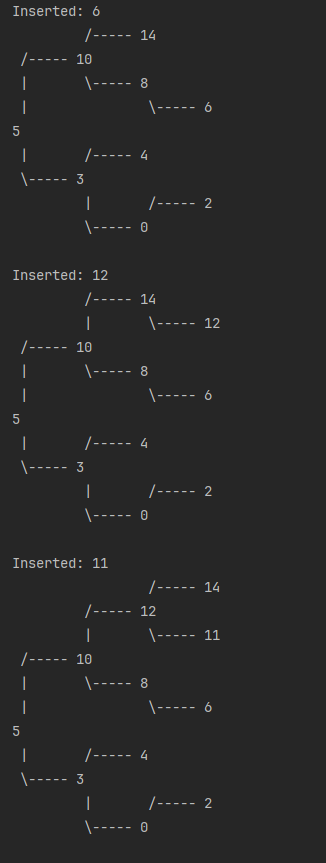
\includegraphics[scale=0.7]{images/result3.png}
        \caption{Последни 3 добавяния в дървото}
\end{figure}
\noindent
По същия начин при добавяне на 11 се случва балансиране, защото лявото поддърво на 14 става по-висок от останалите. 






















\end{document}